OLD LIT NOTES

KAMALI
Kamali developed a model for an automated platoon, defining procedures for vehicles joining and leaving. 

A joining vehicle can integrate at either the back or the middle of the platoon. The vehicle first sends a join request to the platoon leader. If the vehicle is at the back of the platoon the leader sends an agreement and the vehicle follows its predecessor. If the vehicle requests to join in front of another platoon vehicle, the leader first asks the platoon vehicle to increase space; once the space is large enough for the joining vehicle, the leader sends an agreement. The joining vehicle then manoeuvres into the space and follows the preceding vehicle. Having now joined the platoon, the vehicle sends a confirmation to the leader. The leader then requests that the vehicle that gave way for the joining vehicle decreases their spacing back to normal.

A leaving vehicle sends a request to the leader. When it receives permission to leave the vehicle increases its spacing from its predecessor; once the vehicle is at its maximum distance from its predecessor the vehicle can change lanes. Once out of the convoy the vehicle sends an acknowledgement to the leader.

This model isn't very strict, acting as more of a set of requirements than a true model. The paper sets the requirements using pre-defined gaps, and has no strict calculations guiding following characteristics. It could be implemented using spacing rules from both the IDM and Gipps' model, however, by using V2V communication, the lead vehicle can control the actions of all vehicles in its platoon. Instead of using IDM or Gipps' model, the lead vehicle can control the gaps between vehicles so that they all increase and decrease simultaneously. The gaps could be based on the platoon's velocity, perhaps using \eqref{IDMSpacingFunction} from the IDM. By centralising control in this way, vehicle platoons can avoid the traffic shock effect \citep{Daganzo1994}.

ATAGOZIYEV CENTRALISED LANE MERGE
A centralised system for lane changing was described in a paper by Atagoziyev et al. in 2016 \citep{Atagoziyev2016}. This system uses roadside infrastructure to help groups of vehicles change lanes before they reach a 'critical-position', such as a motorway exit or intersection. The vehicles send their position and velocity information to the roadside infrastructure; the system then sends a number of orders to the vehicles such that they safely rearrange themselves into the correct lanes.  Because the distance travelled by the vehicles involved can be large, particularly at high speeds, the system would struggle to use a reservation tile based system as AIM did, instead Atagoziyev's system manages the gaps between vehicles to safely relocate vehicles into the correct position. A more comprehensive overview is given in \ref{subsec:Lane Changing to hit a target lane}.

Atagoziyev's system would only need to be applied during the approach to critical-positions. Vehicles could be managed using platoons or another vehicle following model until that point. A centralised system provides a single communication point which manages all of the vehicles that want to change lanes. This helps to reduce the volume of communications required and creates an entity with a global view of the vehicles' positions and goals. A V2V solution would most likely require more communications and may never obtain a complete picture of the situation, possibly leading to sub-optimal lane changing orders.

Note that Atagoziyev's system could be adapted, such that all of the vehicles communicate with the platoon leader instead of roadside infrastructure. Though this could be called a V2V communication solution, the effective solution is still considered centralised, as all decisions are made by one entity.

GIPPS AND MOBIL DECENT
Cost also becomes a major issue for centralised systems when you consider fast moving situations such as lane changing on a motorway. To implement Atagoziyev's model, vehicles must remain in range of the roadside infrastructure. This would mean that the infrastructure will have to continue on for a long distance, which could become very expensive, especially given the number of critical-positions on a motorway. Decentralised solutions reduce these costs massively.

Two examples of decentralised lane changing models are Gipps' 1986 driver decision model \citep{Gipps1986} and the MOBIL model developed by Kesting et al. in 2007 \citep{Kesting2007}. These models are decentralised and as such do not have to rely on roadside infrastructure in order to change lanes. This greatly reduces the cost of both implementations and allows the vehicles to be more flexible as to when they change lanes, no longer having to wait until they reach the lead up to a critical-position supported by roadside infrastructure. This flexibility means that vehicles could change lanes to increase their average velocity rather than just changing lanes in order to make a turn or leave the motorway at a critical-position. It also allows vehicles to deal with unexpected situations far from any roadside infrastructure. For example, a broken down car blocking a lane can be evaded. There is more information on Gipps' 1986 model and MOBIL in \ref{sec:Making lane changing decisions}.

GIPPS 1986
In 1986 Gipps' modelled driver behaviour in real world circumstances, characterising the decisions a driver has to make in order to determine whether to change lanes \citep{Gipps1986}. The paper was designed to be used with the Gipps' 1981 car-following model \citep{Gipps1981}, explained in \ref{sec:Car Following Models}.

The model itself is constructed as a flow chart, in which the decision nodes are the choices a driver must make.You can see the flowchart in Figure \ref{fig:Gipps1986Flowchart}.

\begin{figure}[htb]
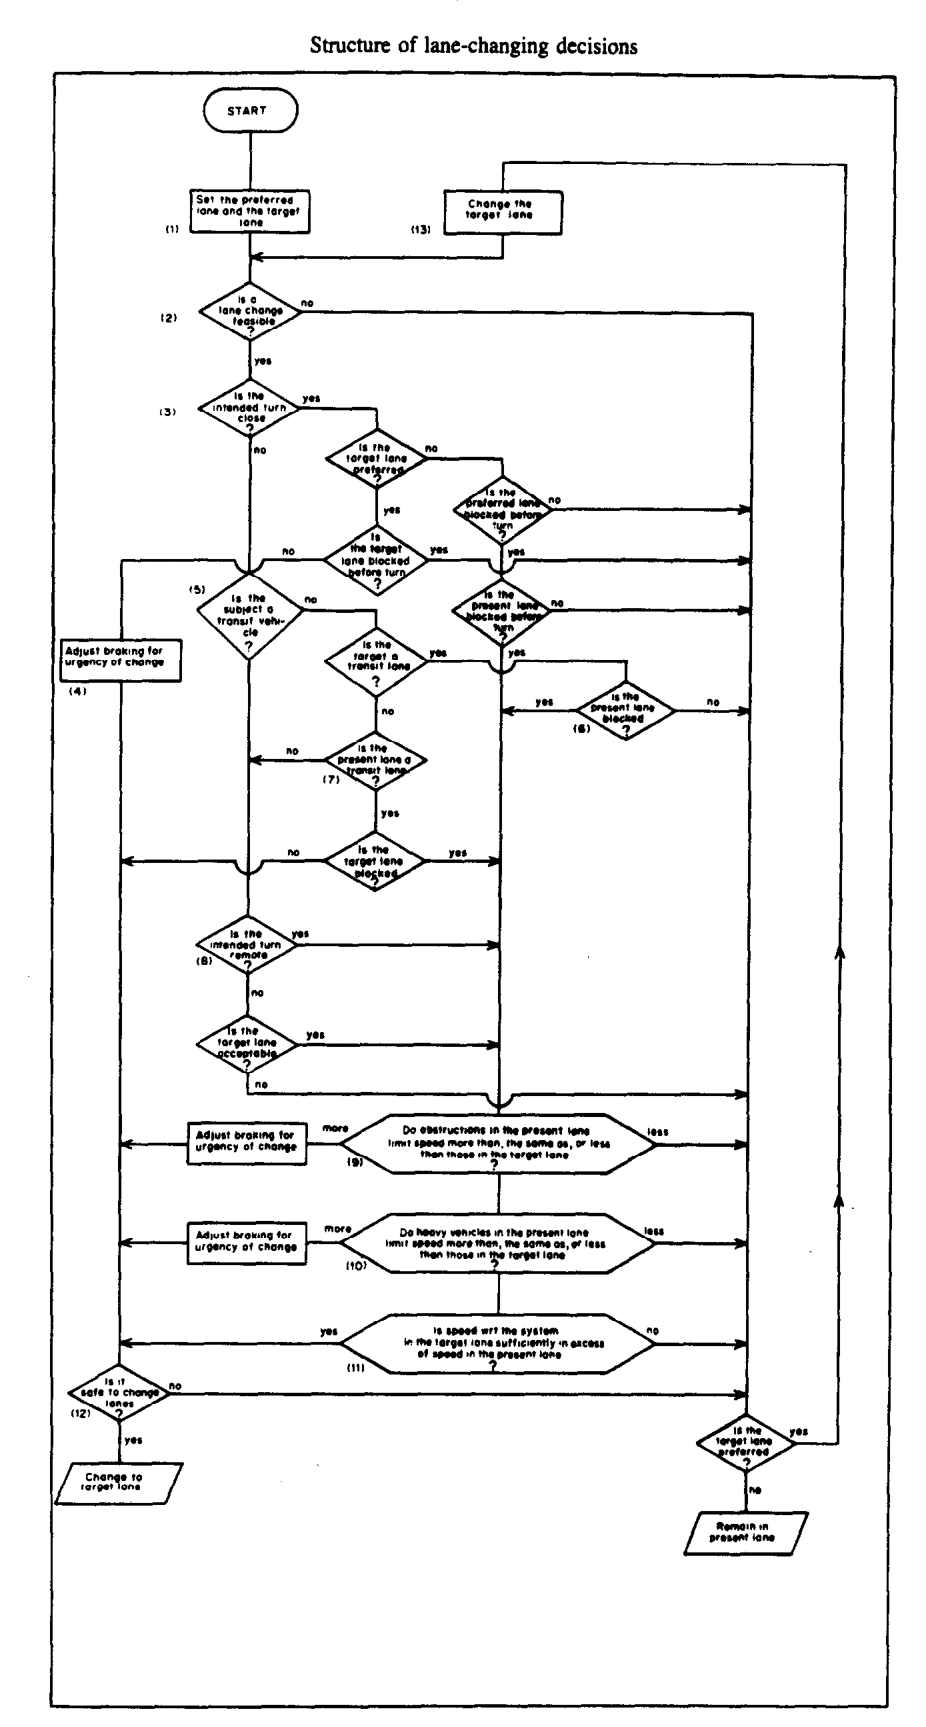
\includegraphics[width=\textwidth]{litReview/gipps1986Flowchart.png}
\caption{The flowchart for lane changing decisions from \citep{Gipps1986}}
\label{fig:Gipps1986Flowchart}
\end{figure}

After determining whether a lane change is feasible the model considers whether the driver needs to move into another lane because they are heading towards a critical point.

These decisions are modelled in nodes 3 and 4.

\begin{enumerate}
\item[3] \textit{Driver behaviour close to the intended turn}

If the driver is close to their intended turn then they will always attempt to change into their preferred lane. Only if blocked will they consider moving into another lane. 

'Close' varies depending on regional differences and the level of traffic, but in the model, close is defined as the driver being within a distance equal to ten seconds of travel from the turn at the driver's desired speed.

\item[4] \textit{Urgency of changing lanes}

The urgency of changing lanes increases as the driver gets closer to their turn. The willingness of the driver to brake harder and accept smaller gaps increases as the driver gets closer to their intended turn.

In the implementation, the braking rate a driver is willing to when first becoming close doubles by the time the intended turn is reached. 

\begin{itemize}
\item[$D_n$] is the location of the intended turn
\item[$V_n$] is the desired (or free) speed of the driver
\item[$b_n^*$] is the most severe braking the driver would otherwise be willing to undertake
\end{itemize}

\begin{equation}
b_n = \Biggl[2 - V_n\frac{(D_n - x_n(t))}{10}\Biggr]b_n^*
\end{equation}

\end{enumerate}

Similarly to Gipps 1981 car-following model, this driver decision model is based on human driver behaviour and as such falls into similar pitfalls. There could be more optimal driver behaviours which would ensure that a driver is in the correct lane well before the critical position. However, because Gipps 1986 model is designed to model human driving behaviour we can expect it to perform less than optimally.

GIPPS 1986 2
Gipps' driver decisions model also considered situations where the driver does not have to be in any particular lane. The model considers the effects of transit lanes, heavy vehicles and the effect of the preceding vehicle on the driver's vehicle. These are shown in nodes 5 to 7 and 9 to 11 of Gipps' flowchart in Figure \ref{fig:Gipps1986Flowchart}.

\begin{enumerate}
\item[5] \textit{Transit vehicles and lanes}
Transit lanes are lanes dedicated solely for public transport and other high occupancy vehicles. These include vehicles such as buses, taxis and carpool cars. These vehicles are known in the model as 'transit vehicles'.
\item[6] \textit{Entry of nontransit vehicles into transit lanes}
If there is an obstruction in the present lane, it is often considered to be a valid reason for a non-transit vehicle to enter a transit lane. 
\item[7] \textit{Departure of nontransit vehicles from a transit lane}
Once the obstruction has been cleared, nontransit vehicle must move back into a valid lane. This forced departure does not affect vehicles that are close to their intended turn.
\item[9] \textit{Relative advantages of present and target lanes}
If the driver has not yet been forced to change lanes by any other factors, then they can look at the relative advantages of the present and target lanes, considering obstructions and then determining which lanes obstructions will have the least effect on their safe speed.
\item[10] \textit{The effect of heavy vehicles} 
If obstructions are level with each other or beyond the range a driver considers, then the driver considers the next heavy vehicle in each lane, as if it were the leading vehicle in an ordinary car following situation. The driver then selects the lane which will give them the higher speed.
\item[11] \textit{The effect of the preceding vehicle}
If there are then no heavy vehicles, the driver considers the speed possible in each lane and then changes if they gain a 'sufficient' speed advantage. This is again, subjective, depending on the present lane, target lane and the type of vehicle.
\end{enumerate}

Again, Gipps' 1986 model was built with human drivers in mind, and as such it fails to take advantage of the benefits of autonomous vehicles such as platooning and vehicle-to-vehicle communications.